\documentclass[11pt, a4paper]{article}
%\usepackage{geometry}
\usepackage[inner=1.5cm,outer=1.5cm,top=2.5cm,bottom=2.5cm]{geometry}
\pagestyle{empty}
\usepackage{graphicx}
\usepackage{fancyhdr, lastpage, bbding, pmboxdraw}
\usepackage[usenames,dvipsnames]{color}
\definecolor{darkblue}{rgb}{0,0,.6}
\definecolor{darkred}{rgb}{.7,0,0}
\definecolor{darkgreen}{rgb}{0,.6,0}
\definecolor{red}{rgb}{.98,0,0}
\usepackage[colorlinks,pagebackref,pdfusetitle,urlcolor=darkblue,citecolor=darkblue,linkcolor=darkred,bookmarksnumbered,plainpages=false]{hyperref}
\usepackage{amsfonts}
\usepackage{amsmath}
\usepackage{tikz}
\usetikzlibrary{automata, positioning}
\renewcommand*{\arraystretch}{.5}

%Make ShortHands for quick updates
\renewcommand{\thefootnote}{\fnsymbol{footnote}}
\newcommand{\sems}{{Spring 2018}}
\newcommand{\classNum}{{MATH 3312}}
\newcommand{\prob}{{\mathbb{P}}}


\pagestyle{fancyplain}
\fancyhf{}
\lhead{ \fancyplain{}{\classNum} }
\chead{ \fancyplain{}{\sems} }
\rhead{ \fancyplain{}{Dr. Hannay} }
%\rfoot{\fancyplain{}{page \thepage\ of \pageref{LastPage}}}
\fancyfoot[RO, LE] {page \thepage\ of \pageref{LastPage} }
\thispagestyle{plain}

%%%%%%%%%%%% LISTING %%%
\usepackage{listings}
\usepackage{caption}
\DeclareCaptionFont{white}{\color{white}}
\DeclareCaptionFormat{listing}{\colorbox{gray}{\parbox{\textwidth}{#1#2#3}}}
\captionsetup[lstlisting]{format=listing,labelfont=white,textfont=white}
\usepackage{verbatim} % used to display code
\usepackage{fancyvrb}
\usepackage{acronym}
\usepackage{amsthm}
\VerbatimFootnotes % Required, otherwise verbatim does not work in footnotes!




\definecolor{OliveGreen}{cmyk}{0.64,0,0.95,0.40}
\definecolor{CadetBlue}{cmyk}{0.62,0.57,0.23,0}
\definecolor{lightlightgray}{gray}{0.93}

\definecolor{mygreen}{RGB}{28,172,0} % color values Red, Green, Blue
\definecolor{mylilas}{RGB}{170,55,241}


\lstset{language=Matlab,%
    %basicstyle=\color{red},
    breaklines=true,%
    morekeywords={matlab2tikz},
    keywordstyle=\color{blue},%
    morekeywords=[2]{1}, keywordstyle=[2]{\color{black}},
    identifierstyle=\color{black},%
    stringstyle=\color{mylilas},
    commentstyle=\color{mygreen},%
    showstringspaces=false,%without this there will be a symbol in the places where there is a space
    numbers=left,%
    numberstyle={\tiny \color{black}},% size of the numbers
    numbersep=9pt, % this defines how far the numbers are from the text
    emph=[1]{for,end,break},emphstyle=[1]\color{red}, %some words to emphasise
    %emph=[2]{word1,word2}, emphstyle=[2]{style},    
}

%%%%%%%%%%%%%%%%%%%%%%%%%%%%%%%%%%%%
\begin{document}
\begin{center}
{\Large \underline{\textsc{MATH 3312:  Computational Project}}}
\end{center}
%\date{September 26, 2014}

%\begin{center}
%\rule{6.5in}{0.4pt}
%\begin{minipage}[t]{0.90 \textwidth}
%\textbf{Topic:}  Linear Algebra Project \hspace{2.0in} \textbf{Due Date:}  5/8\\
%\end{minipage}
%\rule{6.5in}{0.4pt}
%\end{center}
%\vspace{.5cm}
%\setlength{\unitlength}{1in}
%\renewcommand{\arraystretch}{2}

\section*{Directions:}
The below questions require the use of scientific computing software. You will most likely want to use Matlab or Julia for this as I have provided some code for your use in those languages. You should compile all your results and plots into a typed report to be turned in electronically on Canvas. 

You are encouraged to use online resources and talk with one another about your projects. However, each person is responsible for writing up their own report. This report should be uploaded to Canvas by 11:55 PM on 5/3/2019. 

\section*{Questions:}
\begin{enumerate}
\item \underline{Leslie Matrices:} 
One application of linear algebra is to age-structured population models in ecology. Let $\vec{x} \in \mathbb{R}^N $ represent the population (number of individuals) in a population in $N$ different age categories. 
Let's consider a concrete example, and say we want to model the population of birds where $N$ are the years the bird has been alive. For example, we may have:
\begin{equation}
x^0=
\begin{bmatrix}
100 &
65 &
45 &
33 &
15
\end{bmatrix}^T
\end{equation}
This tells us there are 100 birds which are age 1 (hatched this year), 65 birds which are year 2, etc. Lets use the superscript to indicate how many years have elapsed (so we start with $x^0$ to indicate that is the starting value). This bird species is classified as endangered as we only have $258$ total birds in the population. 

Now we may want to take this data in predict the population in future years. The diagram below shows a graphical version of our model. 
\begin{center}
 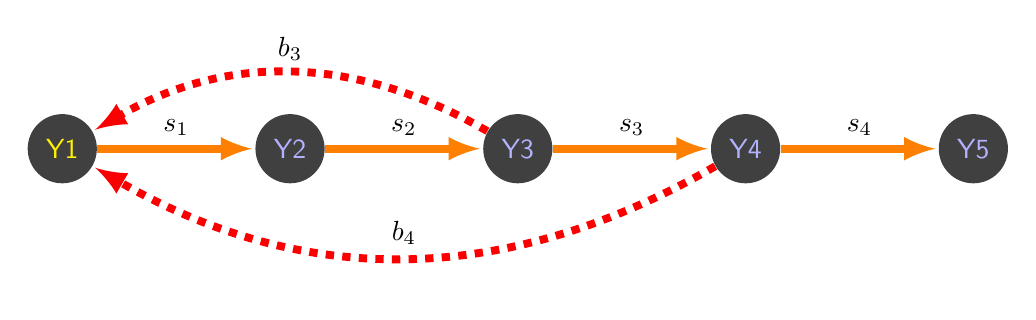
\begin{tikzpicture}[font=\sffamily]
    \node[state,
          text=yellow,
          draw=none,
          fill=gray!50!black] (y1) {Y1};
    \node[state,
          right=2cm of y1,
          text=blue!30!white, 
          draw=none, 
          fill=gray!50!black] (y2) {Y2};
          
         \node[state,
          right=2cm of y2,
          text=blue!30!white, 
          draw=none, 
          fill=gray!50!black] (y3) {Y3};
          
         \node[state,
          right=2cm of y3,
          text=blue!30!white, 
          draw=none, 
          fill=gray!50!black] (y4) {Y4};
          
           \node[state,
          right=2cm of y4,
          text=blue!30!white, 
          draw=none, 
          fill=gray!50!black] (y5) {Y5};
 
    % Connect the states with arrows
    \draw[every loop,
          auto=right,
          line width=1mm,
          >=latex,
          draw=orange,
          fill=orange]
        (y1) edge[auto=left]  node {$s_{1}$} (y2)
        (y2) edge[auto=left]  node {$s_{2}$} (y3)
        (y3) edge[auto=left]  node {$s_{3}$} (y4)
        (y4) edge[auto=left]  node {$s_{4}$} (y5)
        (y3) edge[bend right, auto=right, draw=red, style=dashed] node {$b_{3}$} (y1)
         (y4) edge[bend left, auto=right, draw=red, style=dashed] node {$b_{4}$} (y1);
%        (s) edge[loop above]             node {0.4} (s)
%        (r) edge[loop above]             node {0.3} (r);
\end{tikzpicture}
\end{center}





The $\{Y1,Y2, ...\}$ nodes show the states of being a first year bird, etc. The arrows show the allowed transitions between the states. Lets start with the orange (solid) arrows. They give the fraction of the population which survives the year. For instance, $s_{1}$ gives the fraction of first year birds who survive to be a second year bird. 

The red (dashed) arrows indicate the breeding process. $b_3$ is the average number of baby birds produced by a third year bird in a given year, and $b_4$ is the average number of baby birds produced by a fourth year bird. Evidently, for the species of bird we are studying they can only reproduce in their third and fourth years of life. Perhaps, when they are in their first and second years they are to young and those who are fifth year birds are too old. 

We can translate this graphical version in to a matrix model for our bird population where the can predict the age structured population after $t$ years using the previous year $x^{t-1}$
\begin{equation}
x^{t}=Lx^{t-1} \\
\end{equation}
where $L$ is a matrix called the \textit{Leslie Matrix} for the population:
\begin{equation}
L=
\begin{bmatrix}
0 & 0 & b_3 & b_4 & 0 \\
s_1 & 0 &0 &0 &0 \\
0 & s_2 &0 &0 &0 \\
0 &0 & s_3 &0 & 0 \\
0 &0 & 0 & s_4 & 0 
\end{bmatrix}
\end{equation}

Using the bird population model above answer the following questions:

\begin{enumerate}
\item If $b_3=b_4=2$ and $s_1=0.20$, $s_2=0.50$ and $s_3=s_4=0.80$ and $x^0$ is as given above, make a graph of the total population (sum of the vector) as a function of time. What happens to the total bird population? \\
The below code will save the population at each time point and make a bar plot of the total population:
\begin{lstlisting}
using Plots, LinearAlgebra
pop=zeros(15,1);
for i=1:15; 
	pop[i]=sum(L^(i-1)*x0)
end
bar(0:14, pop)
\end{lstlisting}
Where $L$ is the $5 \times 5$ Leslie matrix as given above and $x0$ is a column vector of the starting conditions. 
\item For the same parameter values as the first question does it matter what the initial population $x_0$ is? Do all initial conditions lead to the same final state for the total population? Hint: what are the eigenvalues for this matrix?
\item Lets say that a conservation program is put in to place for this bird species, designed to increase the survival of the first year birds. Under this conservation program $s_1=0.60$, with all the other parameters being the same. If we start at the $x^0$ given above what happens to the bird population now over the long term? Make a graph of the total population for the first 20 years.
\begin{lstlisting}
using Plots, LinearAlgebra
pop=zeros(20,1);
for i=1:20
	pop(i)=sum(L2^(i-1)*x0); 
end
bar(0:19, pop)
\end{lstlisting}
\item For the conservation program can you find a initial condition where we start with 258 birds (just like the $x^0$ above) where the birds go extinct? What does this tell you about just using the total population as a measure of the health of a population?
\item Let's say the government cuts the funding for the conservation program after 10 years (starting from $x^0$ above ) because the bird population has recovered enough to no longer be endangered. When the funding is cut $s_1$ drops back to 0.20 again. What will happen to the total bird population over the next ten years after the funding is cut? What lesson can you learn from this simulation? 
\item What is the minimum value of the $0 \leq s_1 \leq 1$ parameter where the bird population will grow over time? 
\end{enumerate}

\item \underline{Image Processing: } 
In this question you will use the \textit{singular value decomposition} to compress an image. I have written a julia notebook to do much of this for you. Open this notebook in JuliaBox and download the strang.png file from Canvas and upload this to your JuliaBox account. 


\begin{enumerate}
\item Use the rank\_approx function to compress the image by dropping all singular values but the first 1,10,20,50 components. Make a portfolio of these images. 
\item How many components do we need to include before the loss of information is no longer apparent to the human eye?
\item Find the svd of the image, and plot the singular values. 
\begin{lstlisting}
using Plots, LinearAlgebra
myImageSVD=svdvalues(YOURIMAGE)
bar(myImageSVD) %this will make a bar plot of the singular values
\end{lstlisting}
\item Can you see how the svd can be used to compress the storage required for image files? Hint: Store just the needed singular vectors and values and compute the full image only when required. 
\end{enumerate}

\item \underline{Random Matrices:} We may generate random matrices in Julia using the command randn(n,n) this will create an $n \times n$ matrix where each entry is drawn from the standard normal distribution. To make sure the variance of these matrices doesn't grow with the size of the matrix we will study matrices of the form A=randn(n,n) $\times 1/\sqrt{n}$. 

It turns out that matrices with random entries have some very predictable properties when we consider the \textit{spectrum} (the eigenvalues) of the matrix. The below Julia code creates a random 1000 by 1000 matrix and plots the eigenvalues in the complex plane (real part on the x-axis and imaginary part on the y axis). 

\lstinputlisting{random_matrix_spectrum.jl}

\begin{enumerate}
\item What shape do the eigenvalues form in the complex plane? How does this depend on the size of the random matrix? Try N=10,20,50,100,500,1000 and include these plots in your report.  What happens as the size of the matrices increases?
\end{enumerate}

%\item \underline{Perturbation Theory for Matrices:}
%Work out first order perturbation theory and observe it effects numerically and analytically. 




\end{enumerate}


%%%%%% THE END 
\end{document} 